\section{Ход работы}

Пользователь $A$ решил передать пользователю $B$ сообщение <<\textbf{терпеливо}>>. В нашем алфавите эти буквы кодируются как представлено в таблице \ref{tbl1}.

\begin{table}[H]
	\centering
	\caption{Кодирование заданного сообщения}
	\begin{tabular}{|c|c|}
		\hline
		Символ & Точка      \\ \hline
		т      & (247, 266) \\ \hline
		е      & (234, 587) \\ \hline
		р      & (243, 87)  \\ \hline
		п      & (240, 442) \\ \hline
		е      & (234, 587) \\ \hline
		л      & (237, 454) \\ \hline
		и      & (236, 39)  \\ \hline
		в      & (229, 151) \\ \hline
		о      & (240, 309) \\ \hline
	\end{tabular}
	\label{tbl1}
\end{table}

Для заданий лабораторной работы выбрана кривая E751 (−1,1) , т.е. $y^2 = x^3 − x +1 \pmod{751}$. Кривая представлена на рисунке \ref{fig:elcurve3}.

\begin{figure}[H]
	\centering
	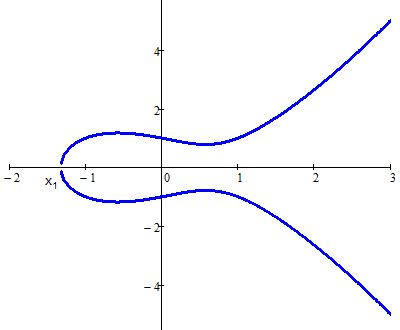
\includegraphics[width=0.7\linewidth]{img/elCurve3}
	\caption{Кривая $y^2 = x^3 − x +1$}
	\label{fig:elcurve3}
\end{figure}


Шифрованный текст имеет вид $C_m = \{ kG, P_m + k \cdot P_b\}$.

Для нахождения $kG$ используем правила сложения точек эллиптической кривой.
\[
x_3 = \lambda^2 - x_1 - x_x \pmod{p} 
\]

\[
y_3 = \lambda(x_1-x_3) -y_1 \pmod{p}
\]


\[
\lambda = 
\begin{cases}
\frac{y_2-y_1}{x_2-x_1}, & P \neq Q\\
\frac{3x^2_1+a}{2y_1}, & P = Q
\end{cases}
\]